\pdfminorversion=6
\pdfinclusioncopyfonts=1
\documentclass[10pt,aspectratio=169,table,usenames,dvipsnames,table]{beamer}

\usetheme[progressbar=frametitle]{metropolis}
\usepackage{appendixnumberbeamer}
\usepackage[english]{babel}

\usepackage{amssymb}
\usepackage{amsmath}
\usepackage{mathtools}
\usepackage{csquotes}
\usepackage{verbatim}
\usepackage{csquotes}
\usepackage{qrcode}
\usepackage{tikz}
\usepackage{pgfplots}
\usepackage{graphicx}
\usetikzlibrary{%
calc,
tikzmark,
decorations.pathreplacing,
decorations.pathmorphing,
shapes,
positioning,
fit,
}
\usepackage[backend=bibtex,style=alphabetic,citestyle=alphabetic,maxbibnames=100,maxcitenames=100]{biblatex} % Enable citeyear

\pgfdeclarelayer{bg}
\pgfsetlayers{bg,main}

\graphicspath{{res/icons/} {res/graphics/}}

% Allow tabular aligning authors
\makeatletter
\long\def\beamer@author[#1]#2{%
  \def\and{\tabularnewline}
  \def\insertauthor{\def\inst{\beamer@insttitle}\def\and{\tabularnewline}%
  \centering
  \begin{tabular}{ll}#2\end{tabular}}%
  \def\beamer@shortauthor{#1}%
  \ifbeamer@autopdfinfo%
    \def\beamer@andstripped{}%
    \beamer@stripands#1 \and\relax
    {\let\inst=\@gobble\let\thanks=\@gobble\def\and{, }\hypersetup{pdfauthor={\beamer@andstripped}}}
  \fi%
}
\makeatother

\title{Crypto Attack Toolkit}

\author{}
\institute{Industrial Software}

\newcommand{\lat}{\mathcal{L}}
\DeclareMathOperator{\LLL}{LLL}
\begin{document}

\pgfmathdeclarefunction{gauss}{2}{%
  \pgfmathparse{1/(#2*sqrt(2*pi))*exp(-((x-#1)^2)/(2*#2^2))}%
}
\pgfmathdeclarefunction{unif}{1}{%
  \pgfmathparse{1/(#1)}%
}

\maketitle

\section{In an ideal world\ldots}

\begin{frame}{The prospect}
  Framework for analyzing, attacking and learning crypto\ldots
  \begin{enumerate}
    \item in CTF challenges
    \item during penetration tests
    \item in weird deployments
    \item with custom implementations
  \end{enumerate}
\end{frame}

\begin{frame}{Cross cutting concerns}
  \begin{itemize}
    \item Uniform interface
    \item Extensible and modular architecture
    \vspace{1em}
    \item Consolidation of common attacks
    \item Progress saving
    \vspace{1em}
    \item Great documentation, readable implementation
    \item Test automation
    \item Tutorials
    \vspace{1em}
    \item Python2 and Python3
  \end{itemize}
\end{frame}

\begin{frame}{Potential Users}
  Useful for
  \begin{itemize}
    \item CTF players
    \item prospective cryptanalysts
    \item penetration testers
  \end{itemize}
\end{frame}

\section{Documentation $\land$ Tutorials}

\begin{frame}{Asymmetric Public-Key Encryption --- RSA}
  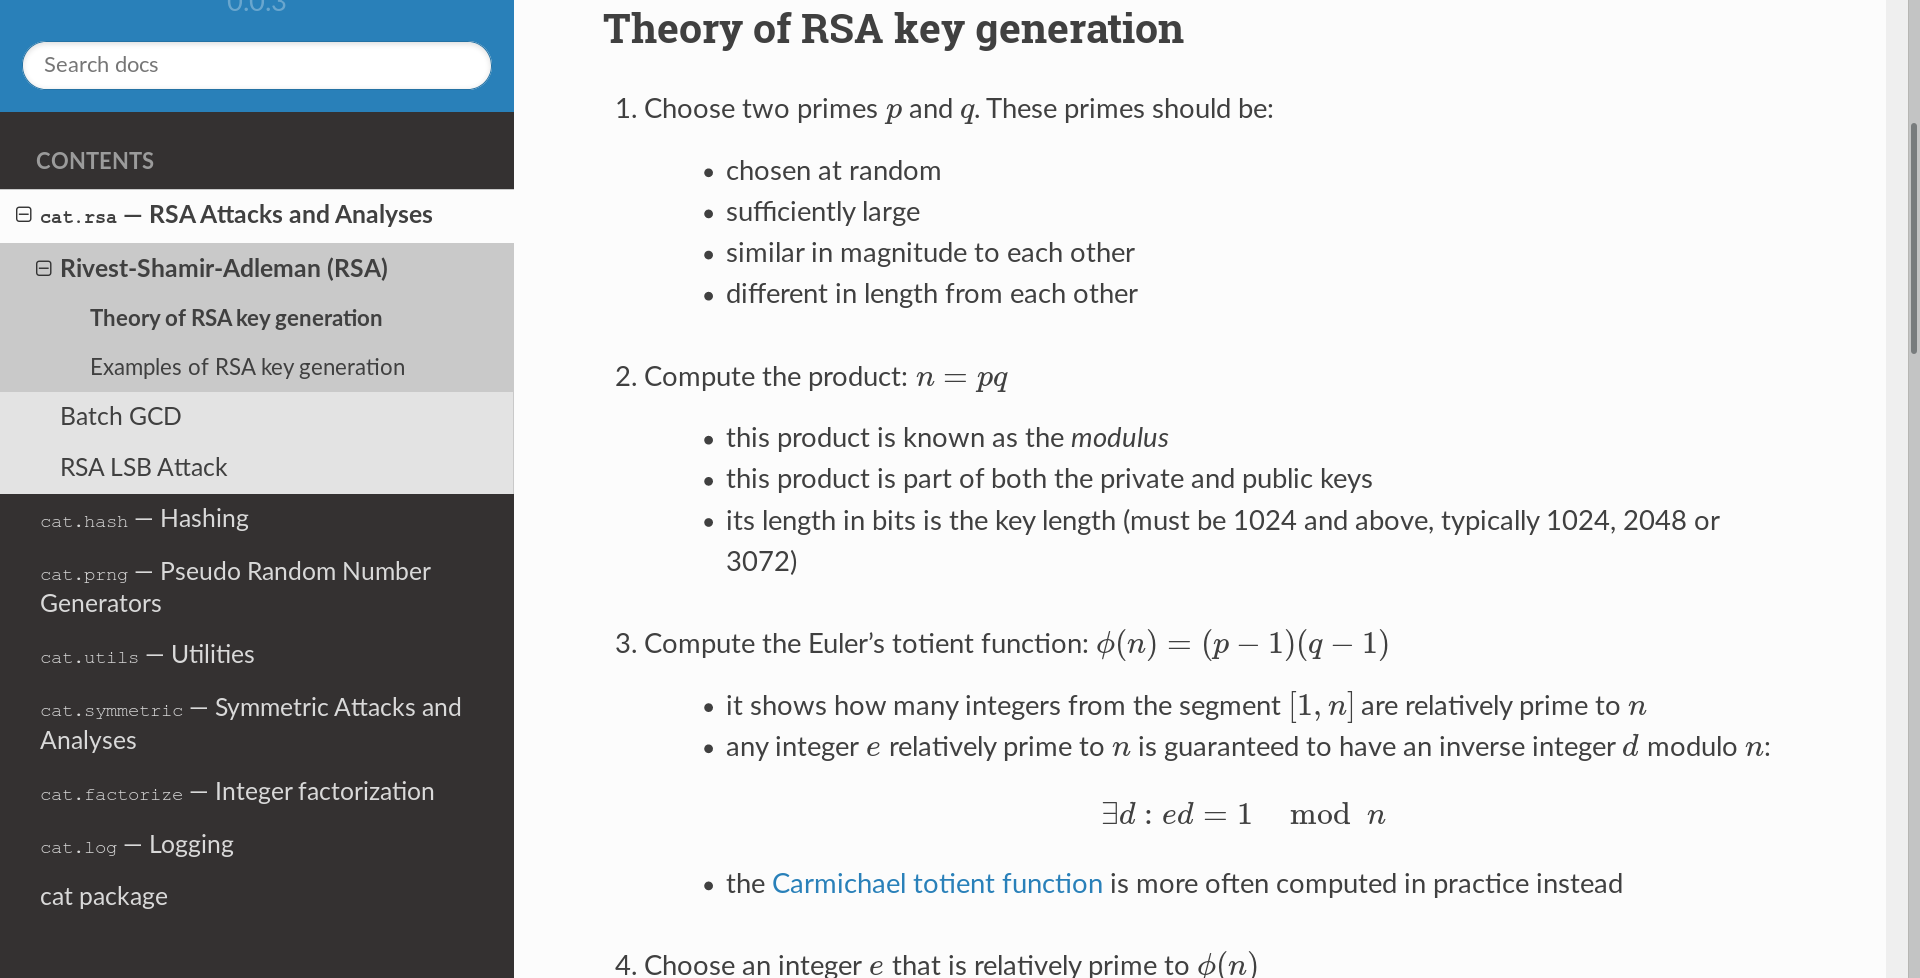
\includegraphics[width=\textwidth, height=0.8\textheight, keepaspectratio]{rsa_doc.png}
\end{frame}

\begin{frame}{Hashing --- Merkle-Damgård Length Extension}
  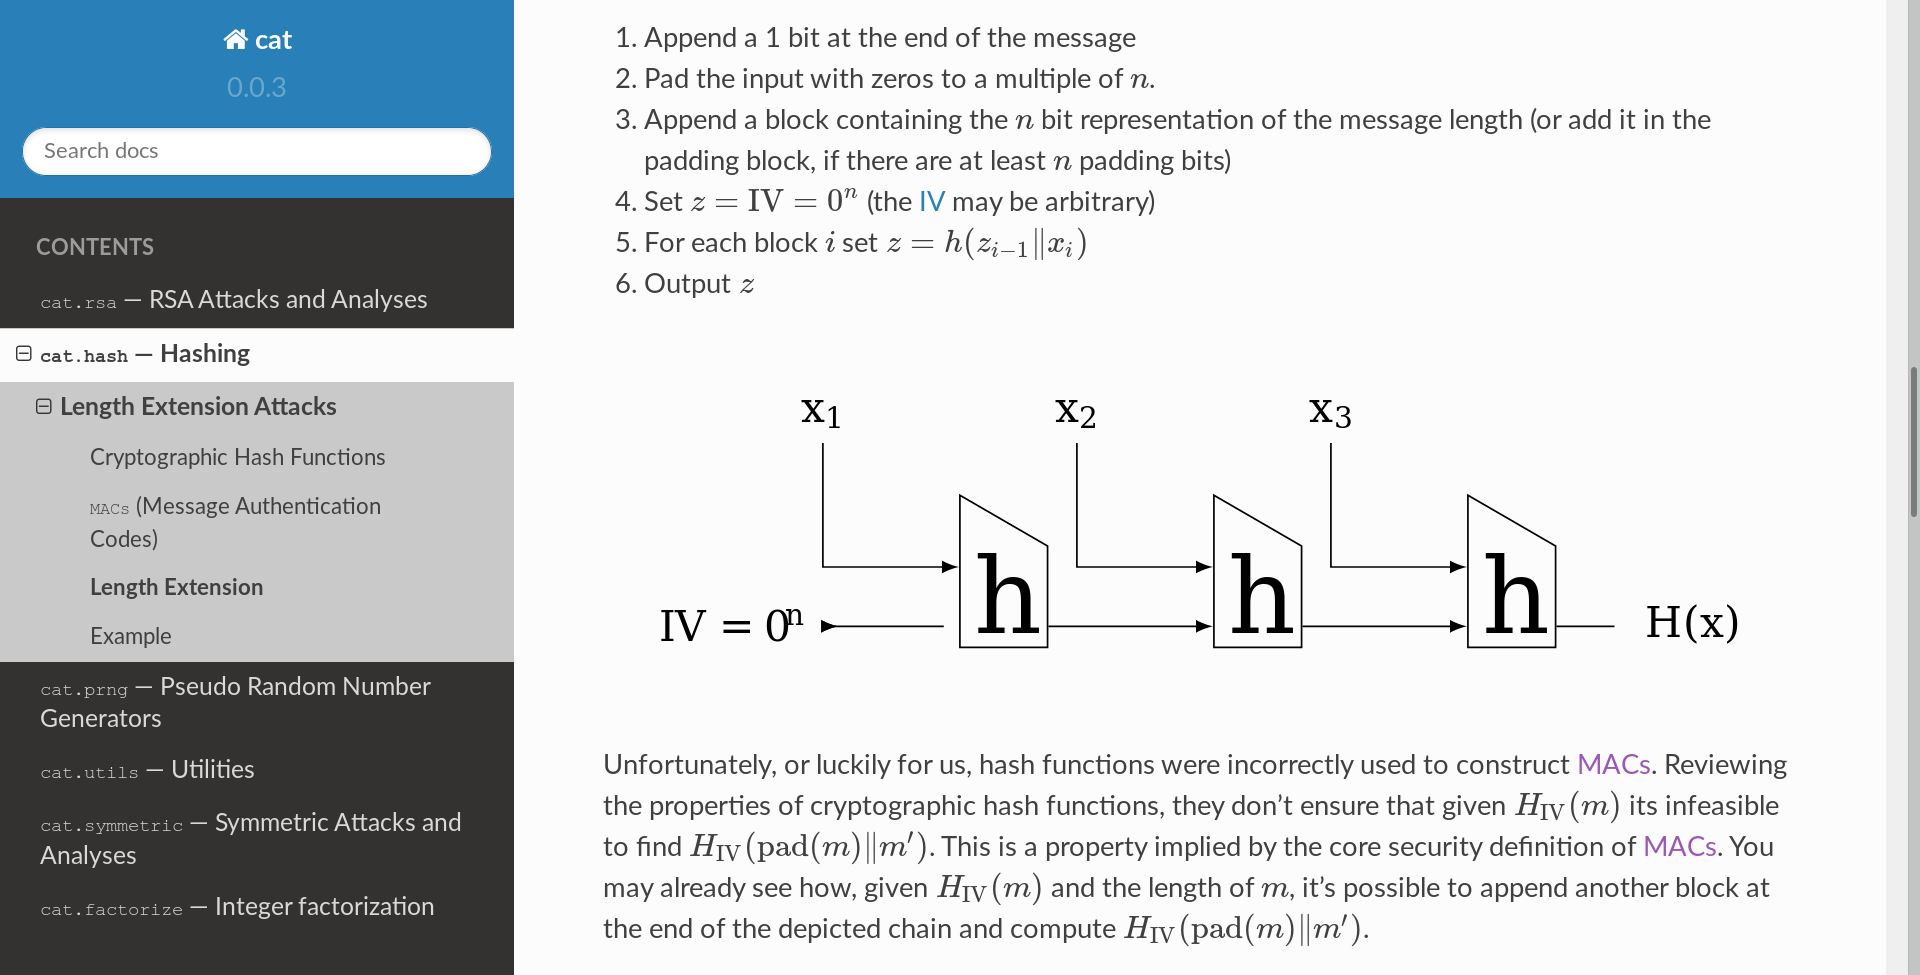
\includegraphics[width=\textwidth, height=0.8\textheight, keepaspectratio]{md_doc.png}
\end{frame}

\begin{frame}{Symmetric Attacks --- Cipher Block Chaining Padding Oracle}
  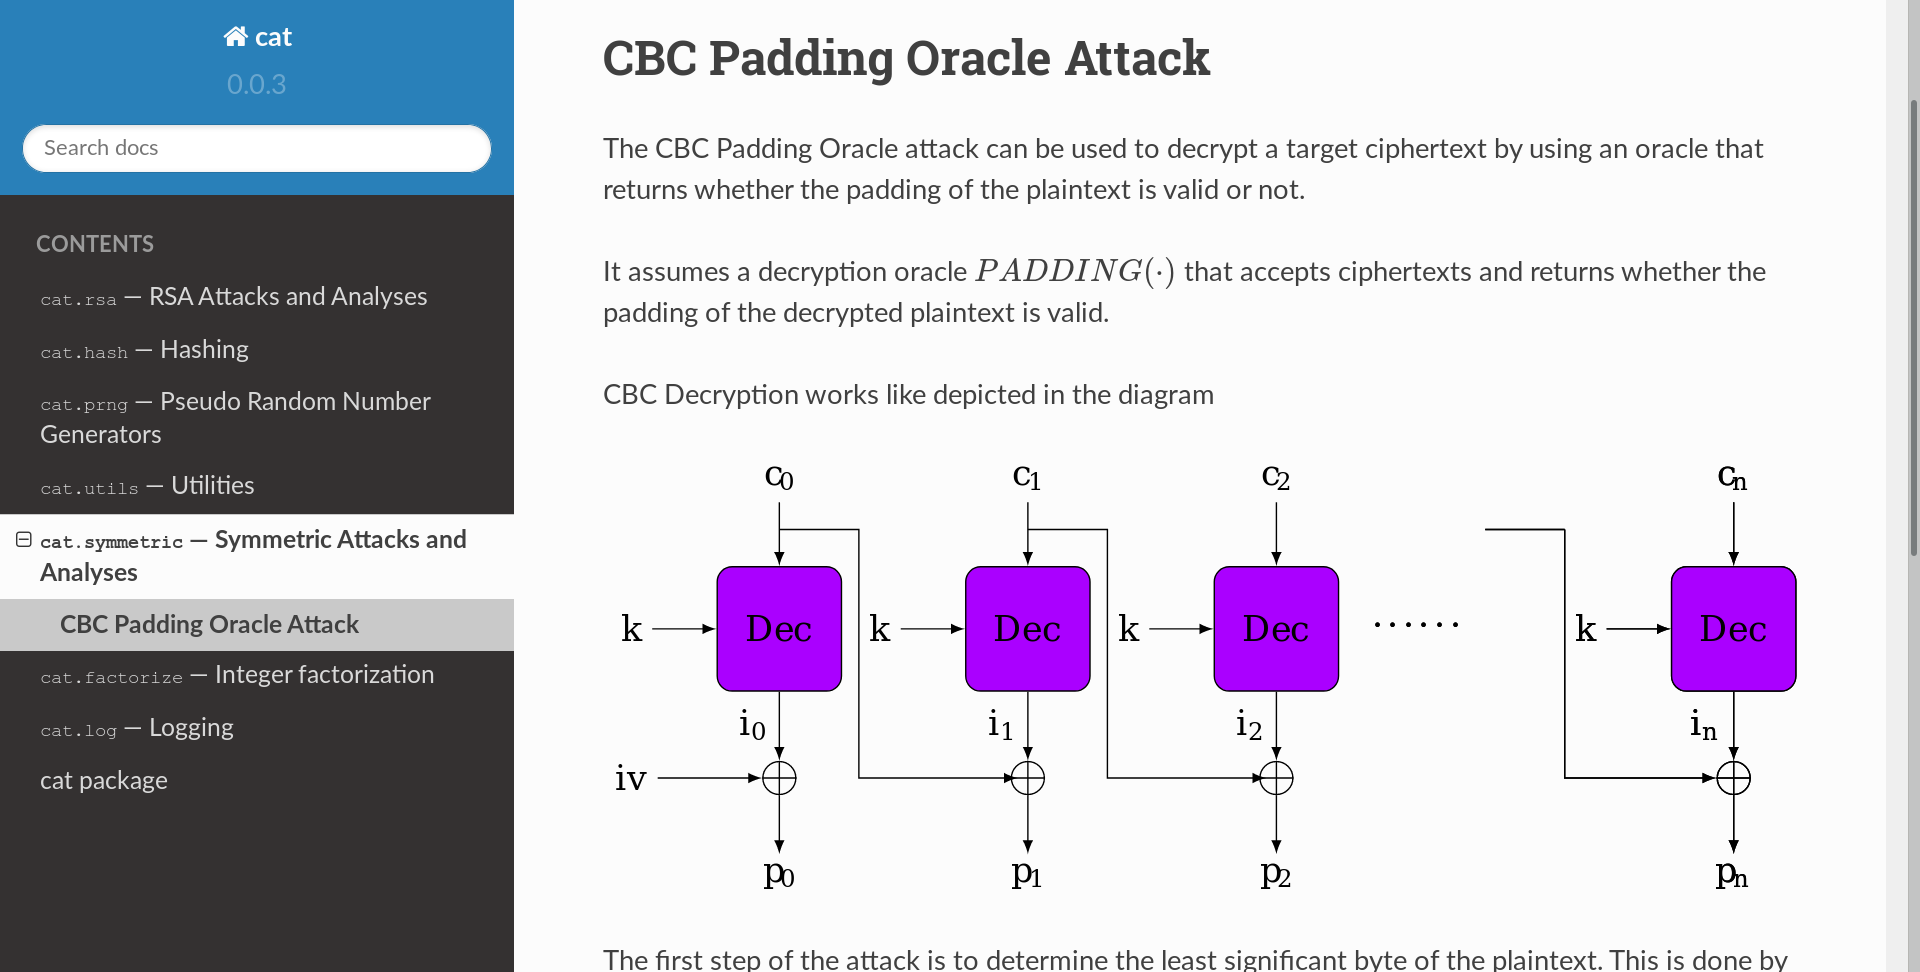
\includegraphics[width=\textwidth, height=0.8\textheight, keepaspectratio]{cbc_doc.png}
\end{frame}

\begin{frame}{Integer Factorization}
  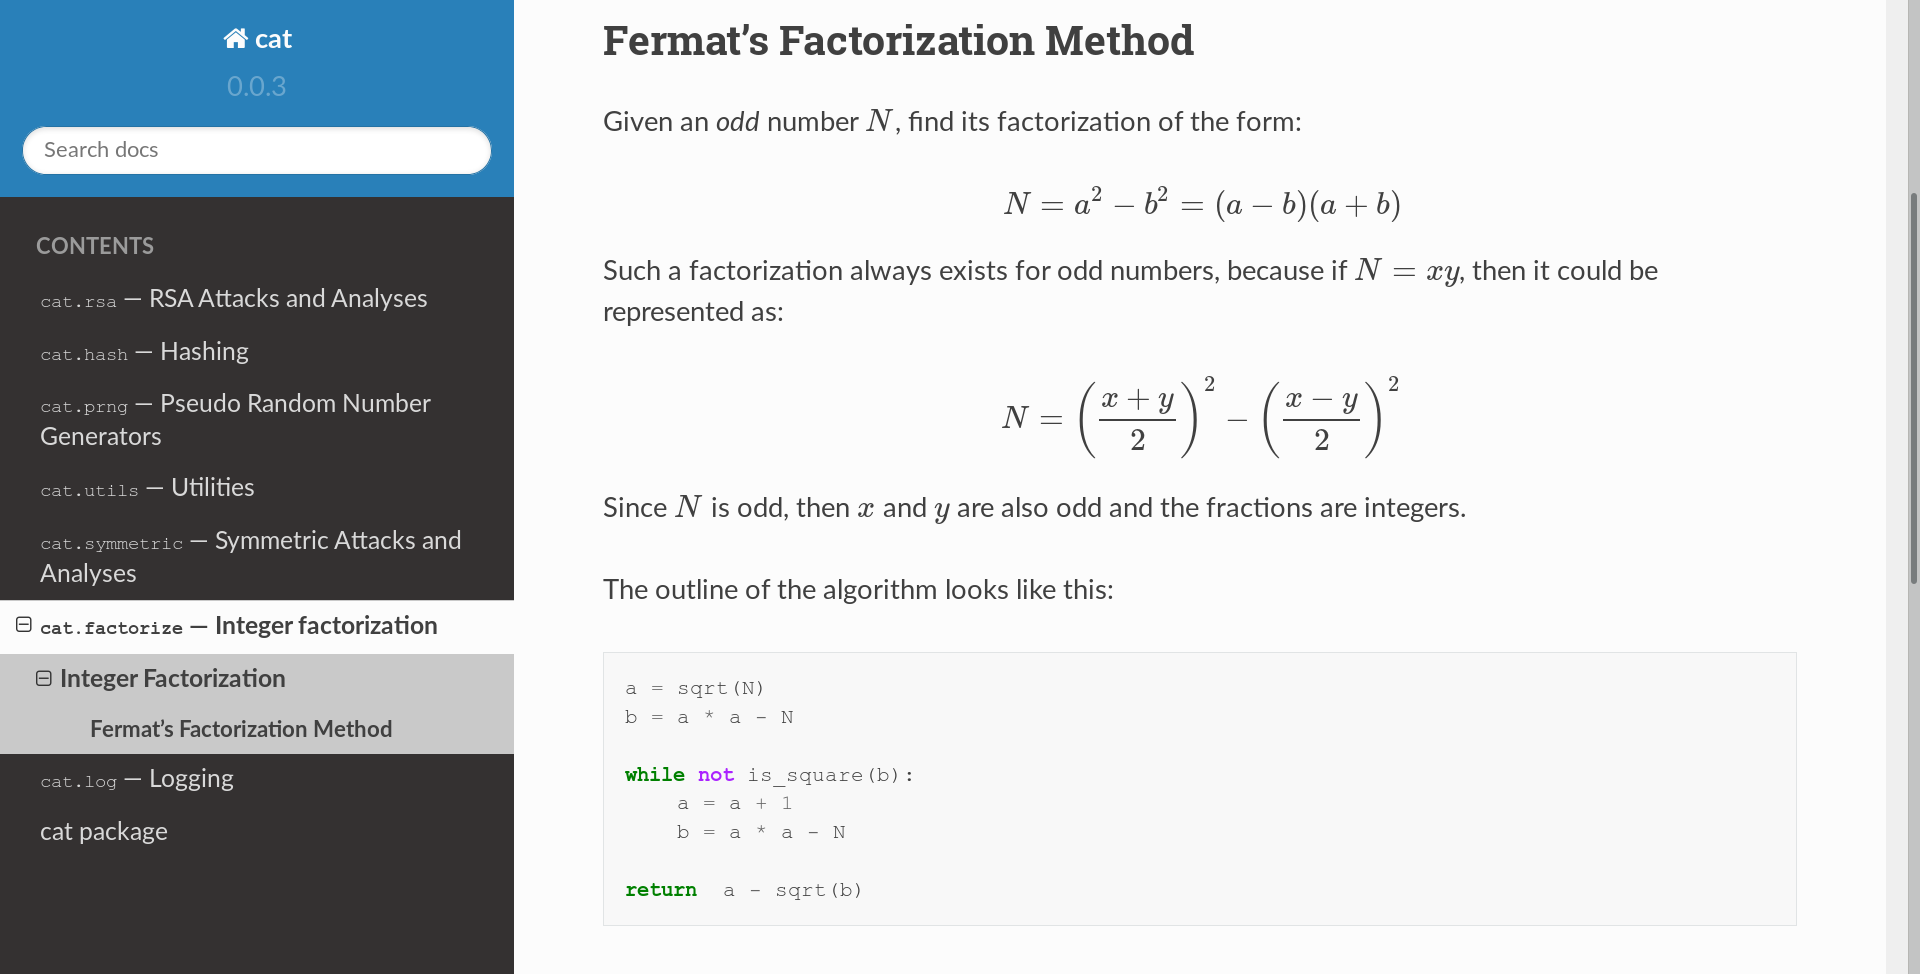
\includegraphics[width=\textwidth, height=0.8\textheight, keepaspectratio]{fermat_doc.png}
\end{frame}

\begin{frame}{Pseudorandom Number Generators --- Linear Congruential Generators}
  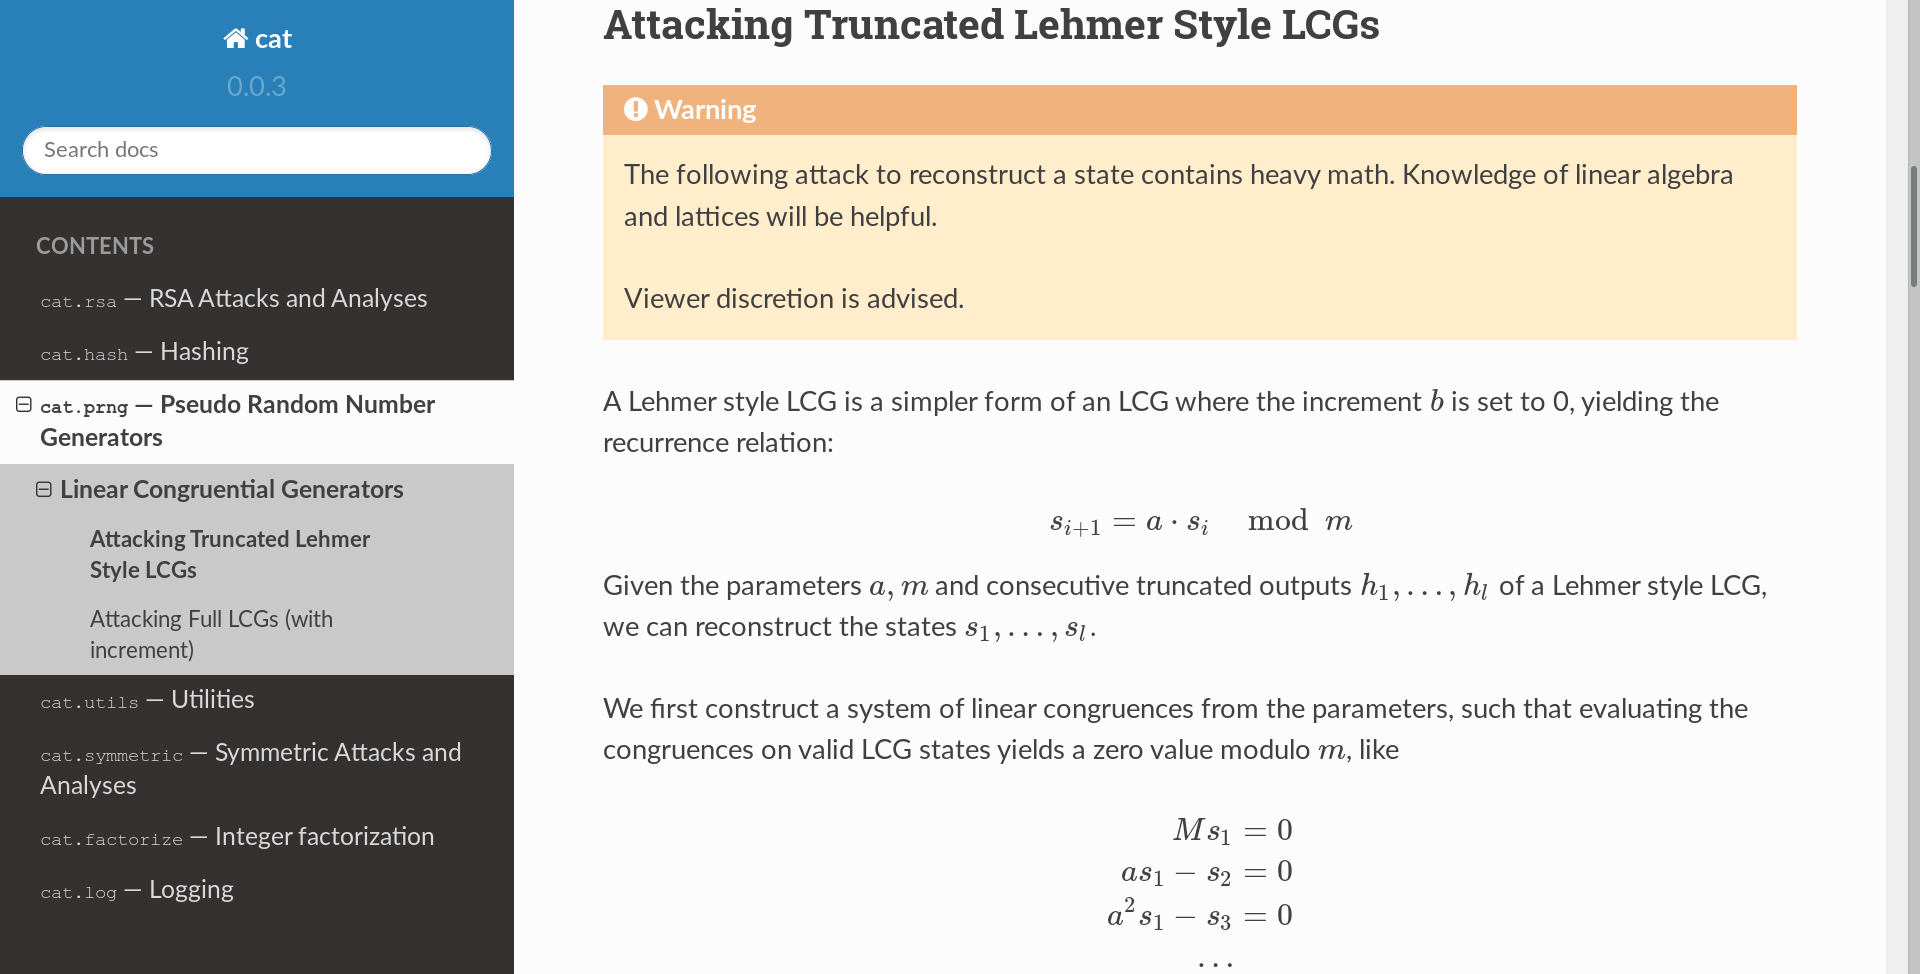
\includegraphics[width=\textwidth, height=0.8\textheight, keepaspectratio]{lcg_doc.png}
\end{frame}

\section{In the real world\ldots}

\begin{frame}{Getting it to build!}
  \begin{itemize}
    \item Needed special functionality
    \item ``Arbitrary'' precision arithmetic
    \item Linear algebra solving
    \item Lattice reductions
    \item Special Hashing
    \vspace{1em}
    \onslide<2->{
    \item Debugging crypto attacks is fun
    \item If a single bit is off, everything looks random
    }
    \vspace{1em}
    \onslide<3->{
    \item and the dead haunted us (Python 2 compatibility)
    }
  \end{itemize}
\end{frame}

\section{Predicting Linear Congruential Generators}

\begin{frame}{Pseudo Random Number Generators}
\begin{minipage}[b]{0.45\linewidth}
  \begin{itemize}
    \item Essentially deterministic machines
    \item We have some ``random'' bits (time, cache misses, TRNGs, \ldots)
      \begin{itemize}
        \item Not necessarily uniform random
        \item Only a few bits of entropy
      \end{itemize}
    \item PRNG takes ``random'' bits as seed and generates
      \begin{itemize}
        \item longer
        \item uniform looking
      \end{itemize}
      bit sequences
  \end{itemize}
\end{minipage}
\hspace{0.5cm}
\begin{minipage}[b]{0.45\linewidth}
\begin{tikzpicture}[thick,scale=0.6, every node/.style={transform shape}]
\begin{axis}[
  no markers, domain=0:10, samples=100,
  axis lines*=left, xlabel=$x$, ylabel=$y$,
  height=5cm, width=7.5cm,
  xtick=\empty, ytick=\empty,
  enlargelimits=false, clip=false, axis on top,
  grid = major
  ]
  \addplot [very thick,cyan!50!black] {gauss(4,1)};
\end{axis}
\end{tikzpicture}
\begin{tikzpicture}[thick,scale=0.6, every node/.style={transform shape}]
\begin{axis}[
  no markers, domain=0:10, samples=100,
  axis lines*=left, xlabel=$x$, ylabel=$y$,
  height=5cm, width=7.5cm,
  xtick=\empty, ytick=\empty,
  enlargelimits=false, clip=false, axis on top,
  grid = major
  ]
  \addplot [very thick,cyan!50!black] {unif(4)};
\end{axis}
\end{tikzpicture}
        \end{minipage}
\end{frame}


\begin{frame}{Linear Congruential Generators}
  \begin{align*}
    s_{i+1} \equiv a s_i + b \mod m
  \end{align*}
  \begin{alignat*}{2}
    m &\in \mathbb{N} \\
    0 \leq a &\leq m \\
    0 \leq b &\leq m \\
    0 \leq s_i &\leq m
  \end{alignat*}
  \begin{center}
    {\large We only get the higher order bits of $s_i$}
  \end{center}
\end{frame}

\begin{frame}{Algebraic Fairy Dust}
  \begin{align*}
    m &\equiv 0 \mod m \\
    a s_1 - s_2 &\equiv 0 \mod m \\
    a^2 s_1 - s_2 &\equiv 0 \mod m \\
    &\vdots \\
    a^n s_1 - s_n &\equiv 0 \mod m \\
  \end{align*}
  \vspace{-2.5em}
  \onslide<2->{
    \begin{align*}
    \onslide<3->{B = \LLL\Bigg(}
    &\begin{pmatrix}
      m & 0 & \cdots & \cdots & \cdots & 0\\
      a & -1 & 0 & \cdots & \cdots & 0\\
      a^2 & 0 & -1 & 0 & \cdots & 0\\
      \vdots & \vdots & \vdots & \vdots & \vdots & \vdots \\
      a^n & 0 & \cdots & \cdots & 0 & -1\\
    \end{pmatrix}
    \onslide<3->{\Bigg)}
    \end{align*}
  }
  \onslide<4->{
  \begin{tikzpicture}[overlay, remember picture]
  \node[anchor=center, scale=1.5, rotate=15] at (current page.center) {
  \begin{beamercolorbox}[center]{title}
    \centering \LARGE
    Use $B$ and higher bits to reconstruct $\vec{s}$
    \end{beamercolorbox}};
  \end{tikzpicture}
  }
  \onslide<5->{
  \begin{tikzpicture}[overlay, remember picture]
  \node[anchor=center, scale=2, rotate=-15] at (current page.center) {
  \begin{beamercolorbox}[center]{title}
    \centering \LARGE
    No one cares. Do the demo
    \end{beamercolorbox}};
  \end{tikzpicture}
  }
\end{frame}

\begin{frame}{We are live!}
  \begin{minipage}{0.5\textwidth}
  \begin{center}
    \qrcode{https://crave.gitlab.io/cat}\\[1em]
    https://crave.gitlab.io/cat/

    Documentation
  \end{center}
  \end{minipage}%
  \begin{minipage}{0.5\textwidth}
  \begin{center}
    \qrcode{https://gitlab.com/crave/cat/}\\[1em]
    https://gitlab.com/crave/cat/

    Source Code
  \end{center}
\end{minipage}
\end{frame}

\end{document}

